\documentclass[11pt,letterpaper]{article}
\usepackage[utf8]{inputenc}
\usepackage{graphicx}
\usepackage{geometry}
\usepackage{booktabs}
\usepackage{amsmath}
\usepackage{amsfonts}
\usepackage{amssymb}
\usepackage{enumitem}
\usepackage{hyperref}
\usepackage{tabularx}
\geometry{left=1.0in,right=1.0in,top=1.0in,bottom=1.0in}
\title{Project Report 1}
\date{February 1, 2023}
\author{Zesen Zhuang}
\begin{document}
\maketitle

\setlength{\parindent}{0pt}
\setlength{\parskip}{0.5em}

\section*{Task 1}

\begin{table}[h]
    \centering
    \begin{tabular}{c c c}
        \hline
        \textbf{Metric} & \textbf{Value} \\
        \hline
        Min             & 0              \\
        Average         & 234,408.55     \\
        Max             & 10,435,467     \\
        \hline
    \end{tabular}
    \caption{Statistics for original data}
    \label{tab:original}
\end{table}

Table \ref{tab:original} shows the statistics for the original data.

\begin{table}[h]
    \centering
    \begin{tabular}{c c c}
        \hline
        \textbf{Metric} & \textbf{Value} \\
        \hline
        Min             & 107,582        \\
        Average         & 226,899.35     \\
        Max             & 349,583        \\
        \hline
    \end{tabular}
    \caption{Statistics for processed data}
    \label{tab:processed}
\end{table}

Table \ref{tab:processed} shows the statistics for the data after removing the outliers.

\subsection*{Outliers detection}

\begin{table}[h]
    \centering
    \begin{tabular}{c c c c}
        \hline
        \textbf{q1} & \textbf{median} & \textbf{q3} & \textbf{iqr} \\ [0.5ex]
        \hline
        198333.0    & 224840.0        & 258834.0    & 60501.0      \\ [1ex]
        \hline
    \end{tabular}
    \caption{Quantiles for the original data}
    \label{tab:quantiles}
\end{table}

Table \ref{tab:quantiles} shows the quantiles for the original data. The interquartile range (IQR) is calculated as $q3 - q1 = 258834.0 - 198333.0 = 60501.0$. The lower and upper bounds are calculated as $q1 - 1.5 \times iqr = 198333.0 - 1.5 \times 60501.0 = 107582.5$ and $q3 + 1.5 \times iqr = 258834.0 + 1.5 \times 60501.0 = 349583.5$. The outliers are defined as the data points that are less than the lower bound or greater than the upper bound. Finally, there are \textbf{559989} songs removed.
\newpage
\section*{Task 2}

\begin{figure}[!htbp]
    \centering
    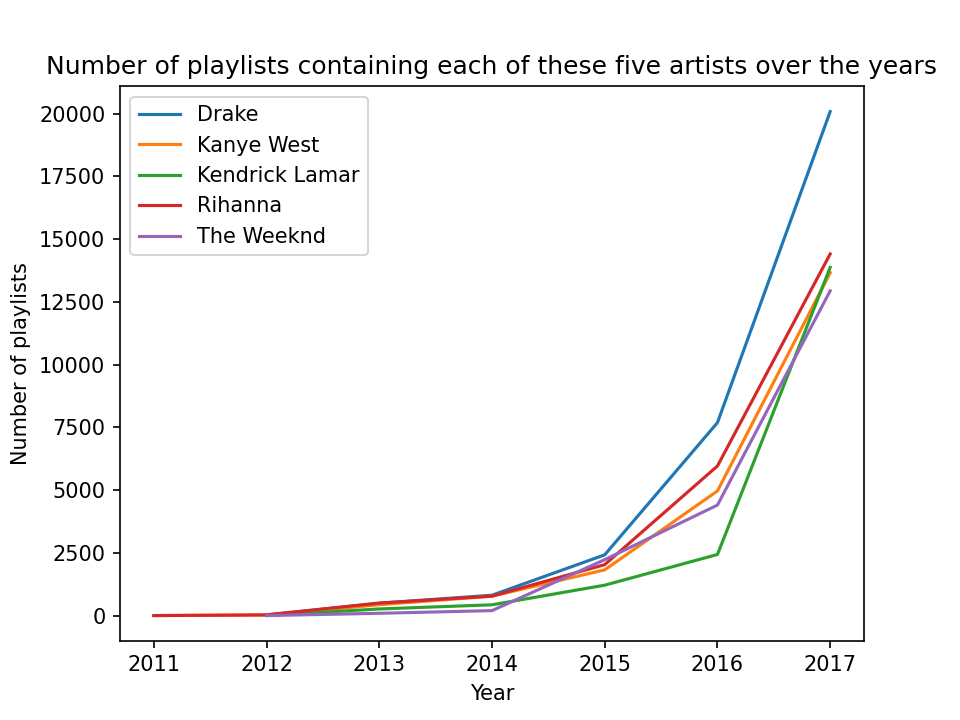
\includegraphics[width=0.5\textwidth]{data/top_5_artist.png}
    \caption{Top 5 artists}
    \label{fig:top_5_artist}
\end{figure}

Figure \ref{fig:top_5_artist} shows the number of playlists containing each of the top 5 artists over the years. The top 5 artists are \textbf{Drake}, \textbf{Kanye West}, \textbf{Kendrick Lamar}, \textbf{Rihanna}, and \textbf{The Weeknd}. \textbf{Drake} is the most popular artist, and all artist have a significant increase in the number of playlists containing them after 2016.

\section*{Task 3}

% Playlist to collect different songs by user preference, musical genre, or a variety of other relationships. In this sense, your task is analyzing how playlists are being created. What is more common, playlists where there are many songs by the same artist or playlists with more diverse songs? To answer this question, compute the prevalence of the most frequent artist in each playlist, defined as the fraction of songs by the most frequent artist. Then create a Cumulative Distribution Function (CDF) plot containing the distribution of artist prevalence across all playlists.

% display data/artist_prevalence_cdf.png

\begin{figure}[!htbp]
    \centering
    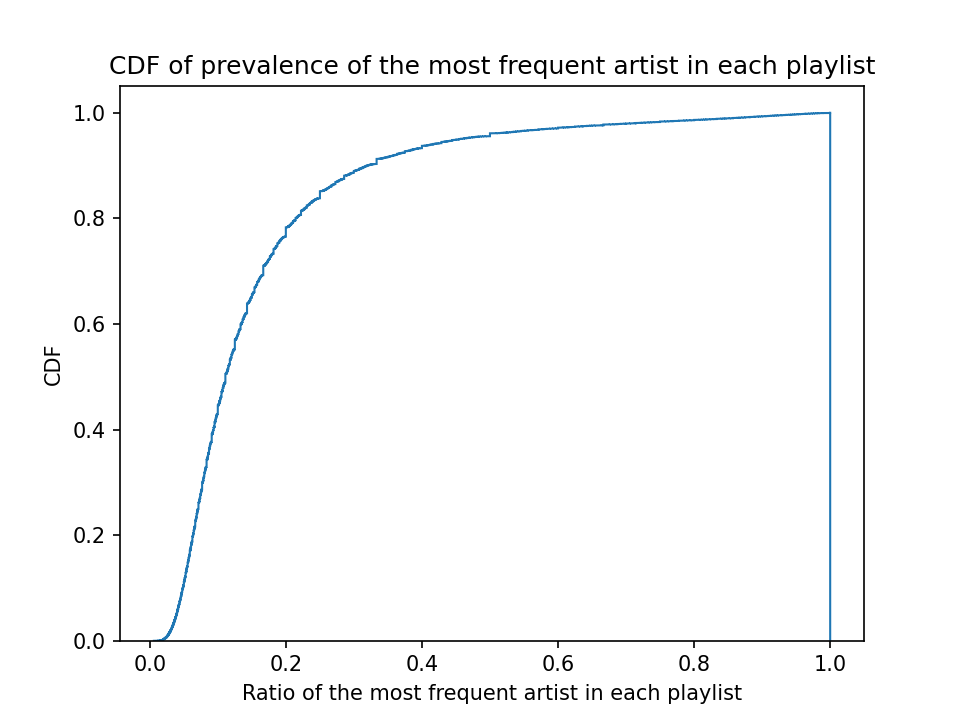
\includegraphics[width=0.5\textwidth]{data/artist_prevalence_cdf.png}
    \caption{Artist prevalence CDF}
    \label{fig:artist_prevalence_cdf}
\end{figure}

Figure \ref{fig:artist_prevalence_cdf} shows the CDF of the artist prevalence. The artist prevalence is defined as the fraction of songs by the most frequent artist. The result shows that most playlists have a low artist prevalence (less than 0.5), which means that the playlists are more diverse.


\end{document}
